\section{Versuchsdurchführung und Auswertung}

\subsection{Verbleibende Aktivität}

Die \Na-Probe wurde laut Beschriftung am Versuchsaufbau am 29.09.1993 eingesetzt. Sie hatte damals eine Aktivität von $A_{93} = 3,7\e{6} Bq$ und die Halbwertszeit wird mit $t_{1/2} = 2,6 a$ angegeben. Somit ergibt sich für die Restaktivität:
\begin{eqnarray*}
 A(t) = & A_{93} \cdot e^{-\frac{\ln 2}{t_{1/2}} t} \\
      \approx & 3,61\e{4} Bq
\end{eqnarray*}
\label{verbleibende_aktivitaet}
Die Messungen in der Staatsexamensarbeit wurden bei $A_{St} = 0,15\, mCurie = 5,55\e{6} Bq$ durchgeführt. Wir erwarten also dass die Rate der Ereignisse im Experiment bei uns in etwa zwei Größenordnungen kleiner sein wird. Für die statistische Genauigkeit der Messungen ist dies nicht von Vorteil.

\subsection{Szintillatorspektren}
Wir haben das Spektrum des \Na  mit jedem der drei Szintillatoren aufgenommen (siehe Abb. \ref{22na-schrottspektrum}). Dazu haben wir je einen direkt an den Multi Channel Analysator (MCA) angeschlossen und 20 min gemessen.

\begin{figure}
 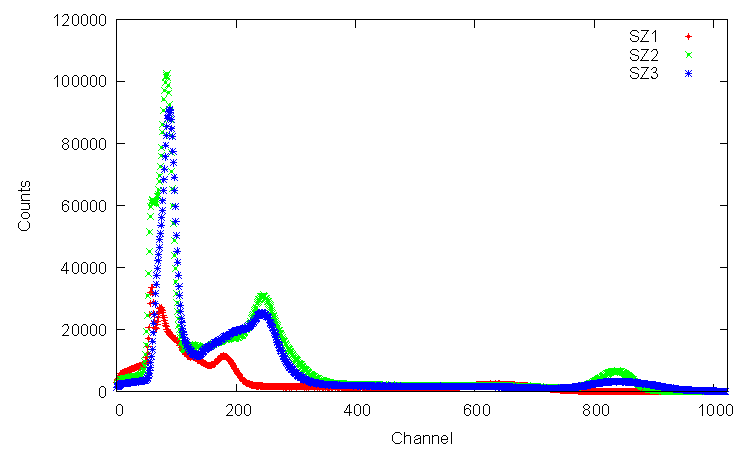
\includegraphics[width=\textwidth]{Graphen/Na-Spektren/na-spektren-1.pdf}
 \caption{Spektrum des \Na-Zerfalls, aufgenommen mit drei ungefilterten Szintilatoren}
 \label{22na-schrottspektrum}
\end{figure}

Dabei haben wir folgende Verstärkungen eingestellt:

\begin{tabular}{lr}
SZ1:& 8,13\\
SZ2:& 5,00\\
SZ3:& 10,00
\end{tabular}


Bei dem kleineren Peak mit hoher Energie (ca. Channel 850) handelt es sich nicht, wie von uns zuerst vermutet, um die 1270keV Gamma-Quanten des \Na-Zerfalls. Vielmehr scheint es sich um einen von der Elektronik erzeugten Störeffekt zu handeln. Der Peak mit der zweithöchsten Energie (Ch.250 bzw. 180) ist dann der eigentliche 1270keV Peak. Die 511keV des Zwei-Photonen-Zerfalls, die Photonen des 3er-Zerfalls und die Bremsstrahlung sind nur schlecht aufgelöst (SZ1 und SZ2) bzw. gar nicht unterscheidbar (SZ3).

Da wir außerdem beim Zuschalten des Single Channel Analysators (SCA) eine Verschiebung des Spektrums beobachteten, haben wir die Energiekalibration dann mit diesem durchgeführt.
\begin{figure}
 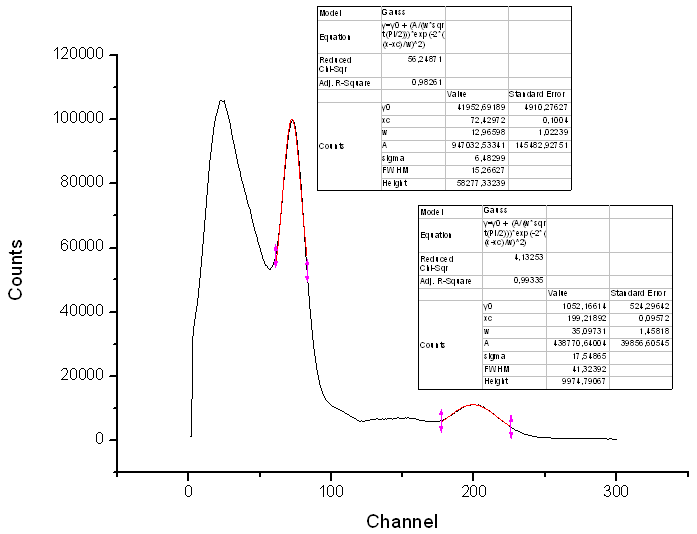
\includegraphics[width=\textwidth]{Graphen/SZ1.png}
 \caption{\Na-Spektrum mit SZ1}
\end{figure}

\begin{figure}
 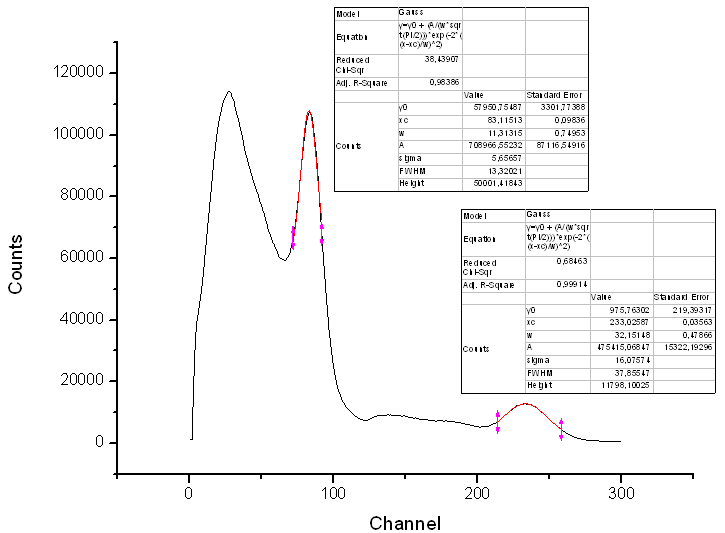
\includegraphics[width=\textwidth]{Graphen/SZ2.png}
 \caption{\Na-Spektrum mit SZ2}
\end{figure}

\begin{figure}
 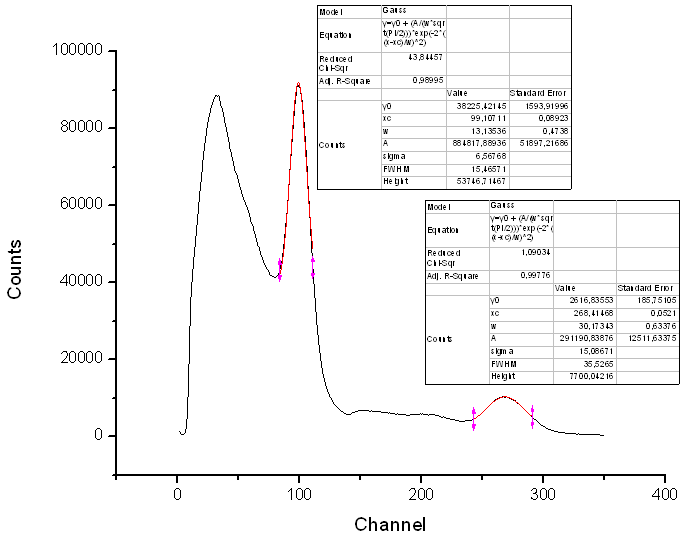
\includegraphics[width=\textwidth]{Graphen/SZ3.png}
 \caption{\Na-Spektrum mit SZ3}
\end{figure}  

Dazu haben wir, wie in Abb \ref{schaltplan_sca_lin_mca} dargestellt, das unipolare Signal des Verstärkers (AMP) zur Einstellung des Energiefensters am SCA verwendet. Liegt ein Ereigniss innerhalb dieses Fensters, so wird ein Signal an das Linear Gate gegeben. Dieses lässt dann für einen kurzen Moment das eigentliche (bipolare) Signal durch. Um die Verzögerung durch den SCA (mindestens ca. $0,05\mu s$) kompensieren zu können, wurde zwischen AMP und Linear Gate noch ein Delay eingebaut. Durch die Verzögerungseinstellung des SCA kann jetzt die Laufzeit beider Signale synchronisiert werden. Dazu wurden der positive Normausgang des SCA und der Ausgang des Delays an die Koinzidenz angeschlossen. Über die feinere Verzögerungseinstellung des SCA wurde die Zählrate maximiert. Anschließend wurden beide Signale an das Linear Gate angeschlossen und dessen Ausgangssignal mit dem MCA analysiert. Das genaue Anpassen der Signallaufzeiten ist wichtig, da sonst einerseits zufällige Ereignisse außerhalb des gewünschten Energiefensters gemessen werden, andererseits aber auch das eigentliche Signal abgeschnitten werden kann. Dies würde dann ebenfalls zu einer falschen Energiemessung führen.

Für eine erneute Messung des \Na-Spektrums haben wir folgende Einstellungen verwendet:
\begin{center}
\begin{tabular}{llll}
\toprule
 & SZ1 & SZ2 & SZ3\\
\midrule
Verstärkung & 8,12 & 10,0 & 10,0\\
Coarse Gain & 20 & 20 & 20\\
Shaping Time & 0,5 $\mu s$ & 0,5 $\mu s$ & 0,5 $\mu s$\\
Lower Level & 0,04 & 0,04 & 0,0\\
Upper Level & 10,02 & 10,02 & 10,0\\
Delay & 2,14 $\mu s$ & 1,83 $\mu s$ & 2,05 $\mu s$\\
Messdauer & 20 min & 20 min & 20 min\\
Delay SCA & 2 $\mu s$ & 2 $\mu s$ & 2 $\mu s$\\
\bottomrule
\end{tabular}
\end{center}

Aus den Spektren haben wir die Position der 511keV- und 1275keV-Peaks abgelesen: %TODO: gauss-fit? 
\begin{center}
\begin{tabular}{lcc}
\toprule
 & 511keV - Peak (Channel) & 1275 keV-Peak (Channel) \\
\midrule
SZ1 & $72,4 \pm 0,1$ & $199,2 \pm 0,1$ \\
SZ2 & $83,1 \pm 0,1$ & $233,0 \pm 0,03$ \\
SZ3 & $99,1 \pm 0,1$ & $268,4 \pm 0,1$ \\
\bottomrule 
\end{tabular}
\end{center}

Somit konnten wir eine Energie-Channel-Eichung für die drei Szintillatoren vornehmen:
%TODO: Fehlerrechnung
\begin{tabular}{ll}
 SZ1 & $E = 6,03 keV \cdot c + 74,77 keV$\\
 SZ2 & $E = 5,10 keV \cdot c + 87,46 keV$\\
 SZ3 & $E = 4,51 keV \cdot c + 63,79 keV$ 
\end{tabular}


\subsection{Zwei-Photonen-Zerfall}

Beim Zerfall des 0S0-Singulett-Zustands des Positroniums können die Photonen, wie in der Theorie näher erläutert, nur in einem $180^\circ$-Winkel abgestrahlt werden. Dies wollen wir über eine Winkelkorrelationsmessung verifizieren. Dazu stellen wir die Szintilatoren auf ein 511keV Fenster ein und drehen SZ1 oder SZ3 gegen den festen SZ2. 

\begin{center}
\begin{tabular}{llll}
\toprule
 & SZ1 & SZ2 & SZ3\\
\midrule
Lower Level & 1,585 & 1,87 & 1,79\\
Upper Level & 2,940 & 3,05 & 3,07\\
511keV Peak & 81  & 80 & 94\\
\bottomrule
\end{tabular}
\end{center}

Die Position des 511keV Peaks zeigt also eine Abhängigkeit von der Einstellung der Energiefenster, insbesondere SZ1 mit $\Delta c_{511} = 8,6$. Dies könnte an einer falschen Delay-Einstellung liegen, der wir aber viel Zeit gewidmet haben, an der besseren Filterung durch den SCA oder an Defekten der Elektronik. Wir haben die Fenstereinstellung mit dem MCA und Computer "`auf Sicht"' vorgenommen und denken, dass wir den 511keV-Peak damit hinreichend genau einstellen konnten, auch wenn er nicht mit der vorher vorgenommenen Energieeichung übereinstimmt.

\subsubsection{SZ2 - SZ3}

Wir haben in $180^\circ$-Stellung von SZ2 und SZ3 die Koinzidenzrate mit der Koinzidenzeinheit optimiert. Dazu haben wir die Rate am Hex-Scaler betrachtet und die Delays angepasst.

\begin{center}
\begin{tabular}{llll}
 & Delay\\
SZ2 & 1,83 $\mu s$\\
SZ3 & 2,83 $\mu s$
\end{tabular}
\end{center}

Um den statistische Fehler möglichst klein zu halten (unter 2\%) berechnen wir die nötige Messzeit pro Winkeleinstellung. Bei $150^\circ$ beträgt die Zählrate etwa $n = 3 Hz$, sodass sich die nötige Dauer wie folgt berechnen läßt:
\begin{equation}
 0,02 = \frac{s_N}{N} = \frac{1}{\sqrt{N}} = \frac{1}{\sqrt{n t}} \Leftrightarrow t = \frac{1}{n}\left( \frac{s_N}{N} \right)^{-2} = 833,3s
\end{equation}
Dies entspricht $t \approx 13,89 \text{min}$. Wir wählen daher eine Messzeit von $t = 16,67 \text{min}$ pro Winkeleinstellung, da sich damit die 100Hz-Clock als Stoppsignal für den Hex-Scaler verwenden lässt (100 000 Counts). 

\begin{figure}
 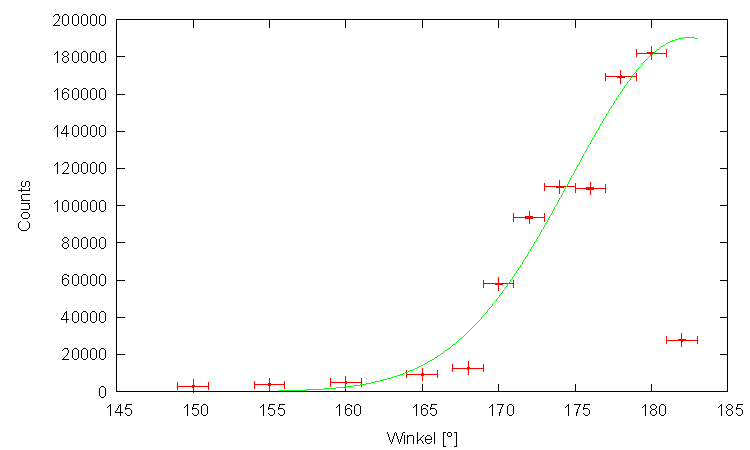
\includegraphics[width=\textwidth]{Graphen/2er/erste.pdf}
 \caption{Winkelkorrelation des Zwei-Photonen-Zerfalls (mit SZ2-SZ3}
\end{figure}

Bei einem Winkel von $182^\circ$ brach die Zählrate leider zusammen. Statt den erwarteten ca. 180 000 Counts erhielten wir nur noch 27 752, also einen Zusammenbruch um eine Größenordnung. Bei einer weiteren Messung stieg die Anzahl zwar wieder etwas, dennoch blieb sie in etwa halb so groß wie erwartet. Dies lag vor allem an einer Reduktion der Zählrate an SZ3 um einen Faktor 5.  

%TODO: Auswertung des Gauß-Fits
%TODO: Untergrund

\subsubsection{SZ2 - SZ1}

Um die Probleme mit SZ3 zu umgehen, haben wir eine erneute Messung mit SZ2-SZ1 durchgeführt. Dabei war die Koinzidenzrate deutlich höher als mit SZ2-SZ3 und somit nicht vergleichbar. Daher haben wir nochmals den kompletten Bereich von $150^\circ$ bis $210^\circ$ untersucht. Eine Messzeit von 100s erschien uns auf Grund der höheren Zählrate ausreichend. (Dies entspricht einem Fehler von ca. 5,8 \% bei $150^\circ$, bzw. 0,6\% bei $180^\circ$)

\begin{figure}
 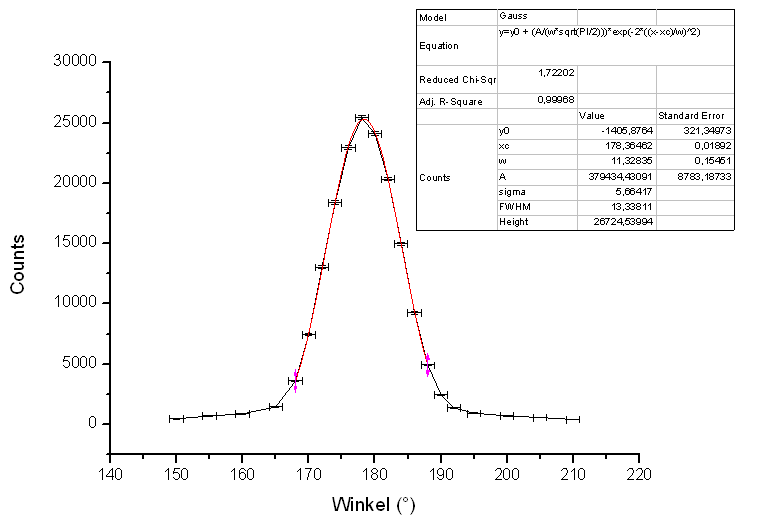
\includegraphics[width=\textwidth]{Graphen/180K.png}
 \caption{Winkelkorrelation des Zwei-Photonen-Zerfalls (mit SZ2-SZ1)}
\end{figure}

Unsere Messungen ergeben also, dass die maximale Zählrate bei $xc = 178,36^\circ \pm 0,01^\circ$ liegt und bestätigt somit die theoretische Aussage, dass der Zwei-Photonen-Zerfall nur in einem Winkel von $180^\circ$ erlaubt ist. Die "`Linienbreite"' von $w = 11^\circ \pm 0,15^\circ$ ergibt sich hauptsächlich aus der Bewegung des Schwerpunktsystems relativ zum Laborsystem. %TODO: Begriffe klären%
%TODO: Abweichung von 180° erläutern

\subsubsection{Zufällige Koinzidenzen}

Um den Anteil der zufälligen Koinzidenzen, also Events die von zwei verschiedenen Zerfällen oder aus Störsignalen herrühren, zu bestimmen haben wir verschiedene Ansätze verfolgt. Zum Einen haben wir sie über die Zählraten und die Zeitauflösung der Koinzidenzeinheit abgeschätzt:
\begin{equation*}
 n_{ZK} = \tau \cdot n_{SZ2} \cdot n_{SZ3} = (0,1262 \pm 0,0057) s^{-1}
\end{equation*}
%Zufällige Koinzidenzen:  0.126152721707
%Fehler:  0.00574067795172

Weiterhin haben wir die Zahl der Koinzidenzen bei senkrechter Stellung der Szintillatoren gemessen:
\begin{equation*}
 n_{ZK-90} = (1,67  \pm  0,13) s^{-1}
\end{equation*}

Zu guter Letzt haben wir wieder die $180^\circ$-Konfiguration eingestellt und das Delay der beiden SCAs gegeneinander verstellt: 
\begin{equation*}
 n_{ZK-delay} = (0,019  \pm  0,004) s^{-1}
\end{equation*}
  
%TODO: was bedeutet das? größte verwenden?

\subsubsection{Austausch von SZ3}
Wir haben die gesamte Elektronik ausführlich untersucht und daraufhin den SCA von SZ3 ausgetauscht, da bei diesem der Pseudo-Peak bei ca 2000 keV viel stärker als bei den anderen beiden war. Weiterhin haben wir die Verstärkung am AMP etwas reduziert, da wir auch ein Übersteuern nicht ausschließen konnten. Danach war zwar das Signal deutlich klarer und der Pseudo-Peak verschwunden. Auf Grund der geänderten Verstärkereinstellungen wurde eine erneute Energie-Kanal-Eichung nötig, die in den Graphen des folgenden Kapitels mit abgebildet ist. 

\subsection{Drei-Photonen-Zerfall}

Bei diesem Versuchsteil geht es zuerst um die Untersuchung des Energiespektrums. Dazu haben wir die Fenster von SCA 1 (Abb \ref{graphen-3er-red-spektrum-sz1}) und SCA 3 (Abb \ref{graphen-3er-red-spektrum-sz3}) so eingestellt, dass nur Events unterhalb der 511keV-Linie registriert werden. Weiterhin haben wir die Signale aller Szintillatoren synchronisiert. Anschließend haben wir über den MCA das Energiespektrum von SZ2 aufgenommen. 
\begin{figure}
 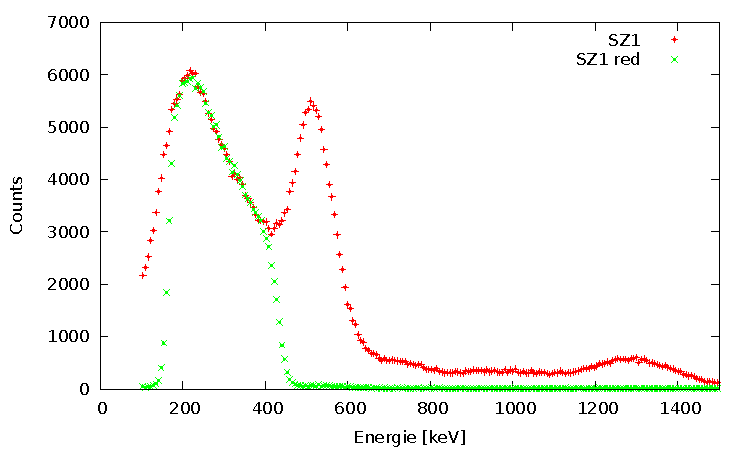
\includegraphics[width=\textwidth]{Graphen/3er/red-spektrum-sz1.pdf}
 \caption{Einstellung des Energiefensters unterhalb der 511keV-Linie für SZ1}
 \label{graphen-3er-red-spektrum-sz1}
\end{figure}


\begin{figure}
 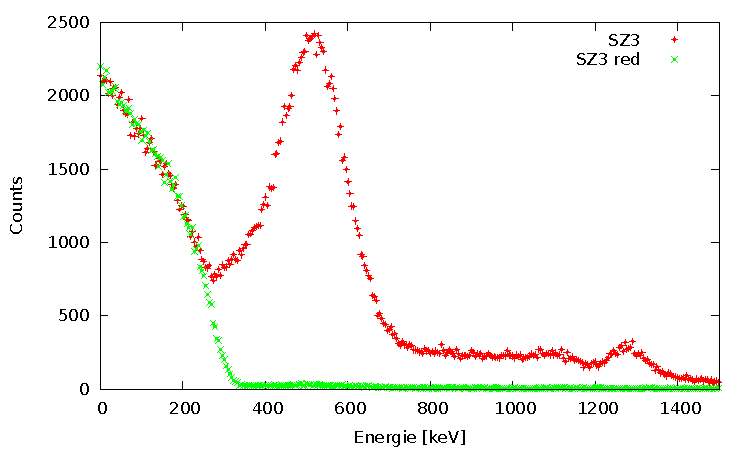
\includegraphics[width=\textwidth]{Graphen/3er/red-spektrum-sz3.pdf}
 \caption{Einstellung des Energiefensters unterhalb der 511keV-Linie für SZ3}
 \label{graphen-3er-red-spektrum-sz3}
\end{figure}

\begin{figure}
 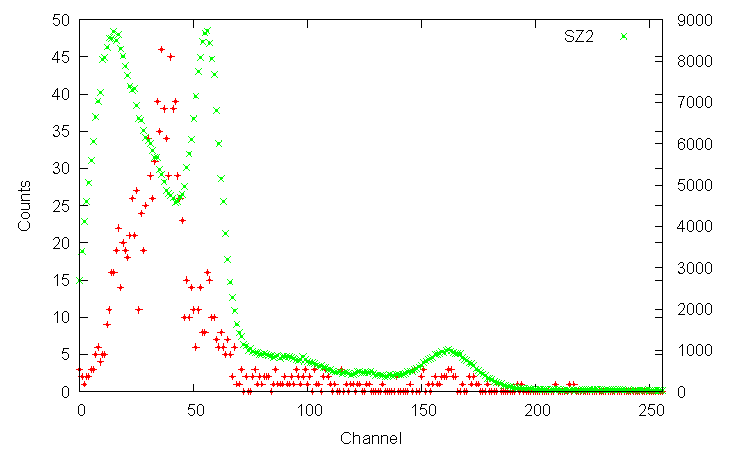
\includegraphics[width=\textwidth]{Graphen/3er/spektrum-2.pdf}
 \caption{Spektrum am SZ2 bei 3er-Koinzidenz}
 \label{graphen-3er-spektrum-2}
\end{figure}

Wir haben dazu eine Messung von ca. 3h Dauer (11091s) durchgeführt. Im Graphen (Abb \ref{graphen-3er-spektrum-2}) haben wir zum Vergleich auch das komplette \Na-Spektrum eingezeichnet. Das Spektrum zeigt ein relativ breites Maximum bei ca. $320-350 keV$.

%TODO: Parameter? Blabla

\begin{figure}
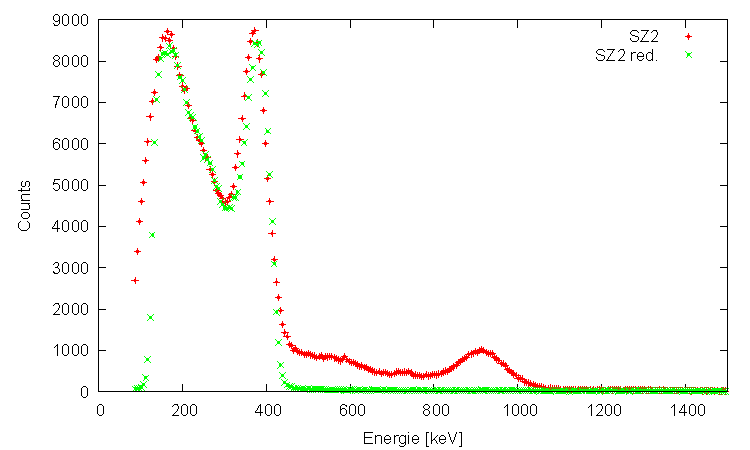
\includegraphics[width=\textwidth]{Graphen/3er/red-spektrum-sz2.pdf}
 \caption{Grobe Einstellung des Energiefensters von SZ2}
\label{graphen-3er-red-spektrum-sz2}
\end{figure}

Für die weiteren Messungen haben wir auch bei SZ2 ein Energiefenster eingestellt, allerdings nur recht grob da die Zählrate auch so schon niedrig war (Abb \ref{graphen-3er-red-spektrum-sz2}). Statt eventuell zulässige Ereignisse von vorneherein zu unterdrücken, haben wir dann lieber bei der Auswertung die Daten etwas beschnitten.

Aus den erneut aufgenommenen \Na-Spektren haben wir die Position der 511keV- und 1275keV-Peaks abgelesen:  
\begin{center}
\begin{tabular}{lcc}
\toprule
 & 511keV - Peak (Channel) & 1275 keV-Peak (Channel) \\
\midrule
SZ1 & $64,04 \pm 0,07$ & $184,2 \pm 3,4$ \\
SZ2 & $55,25 \pm 0,06$ & $161,54 \pm 0,17$ \\
SZ3 & $183,2 \pm 0,2$ & $351,6 \pm 0,6$ \\
\bottomrule 
\end{tabular}
\end{center}

Somit konnten wir eine Energie-Channel-Eichung für die drei Szintillatoren vornehmen:

\begin{tabular}{ll}
 SZ1 & $E = (6,36 \pm 0,18) keV \cdot c + (103,7 \pm 11,6) keV$\\
 SZ2 & $E = (7,19 \pm 0,01) keV \cdot c + (113,9 \pm 0,8) keV$\\
 SZ3 & $E = (4,54 \pm 0,02) keV \cdot c + (-320,4 \pm 3,2) keV$ 
\end{tabular}

Dabei fällt bei SZ3 (Abb \ref{graphen-3er-red-spektrum-sz3}) auf, dass angeblich einige Kanäle des MCA Photonen mit negativer Energie gemessen haben. Dies ist eher unwahrscheinlich und wir vermuten daher zwei Hauptfehlerquellen: einerseits könnten wir die Peaks verwechselt haben. Der 511 keV-Peak müsste dann in der abfallenden Flanke der Bremsstrahlung "`versteckt sein"' (momentan ca. 200keV) und der 1275keV Peak wäre dann der von uns als 511keV angenommene. Die gute Übereinstimmung des Kurvenverlaufs spricht allerdings eher gegen diese These. Eine andere Möglichkeit wäre eine Nichtlinearität, vermutlich bereits direkt in SZ3 oder eventuell auch im Verstärker. Diese erscheint uns wahrscheinlicher. Sollten wir allerdings tatsächlich die Peaks verwechselt haben, würde dies zwar die weitere Messgenauigkeit verschlechtern und zusätzliche Ereignisse erzeugen, nicht jedoch gültige Ereignisse verwerfen.  

\subsection{Quenching}

Beim Quenching untersuchen wir die Abnahme des Drei-Photonen-Zerfalls unter zunehmendem Magnetfeld. Dazu haben wir zweistündige Messungen mit konstantem Magnetfeld durchgeführt und nach je zwei Messungen eine Kontrollmessung ohne Magnetfeld. Diese erlaubt es uns, grobe Drifts und Schwankungen in der Messung zu erkennen und zu kompensieren.

\begin{figure}
 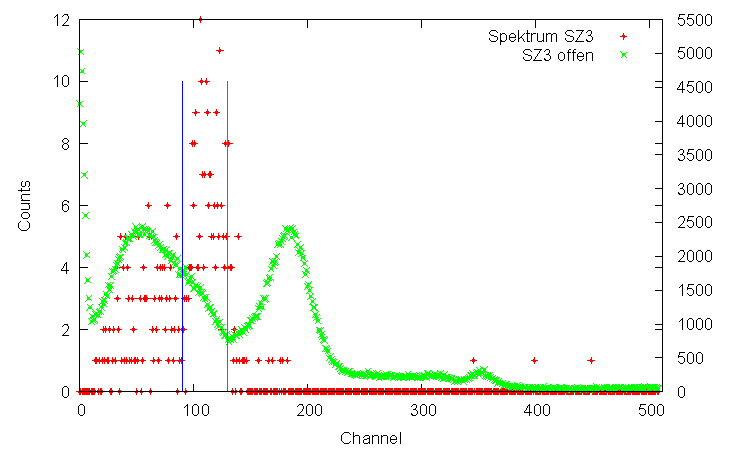
\includegraphics[width=\textwidth]{Graphen/quench/spektrum_0-3.pdf}
 \caption{Spektrum 0,3A}
\end{figure}

\begin{figure}
 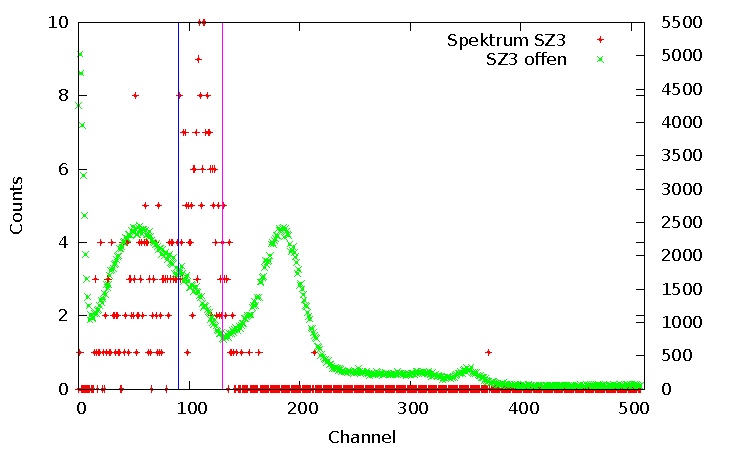
\includegraphics[width=\textwidth]{Graphen/quench/spektrum_1065.pdf}
 \caption{Spektrum 1065G}
\end{figure}


\begin{figure}
 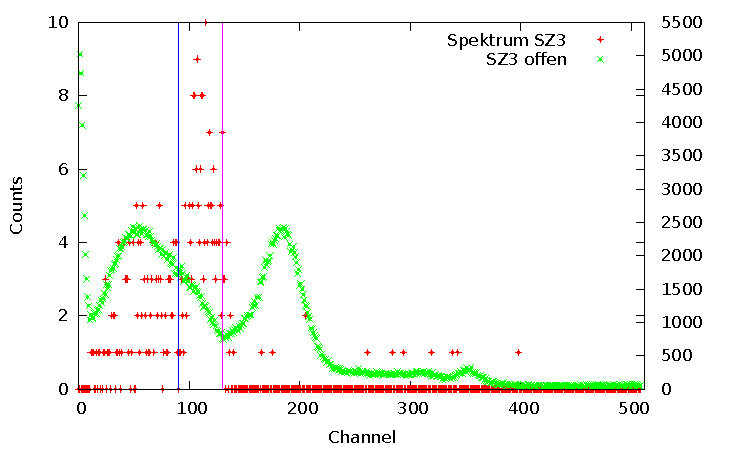
\includegraphics[width=\textwidth]{Graphen/quench/spektrum_2028.pdf}
 \caption{Spektrum 2028G}
\end{figure}


\begin{figure}
 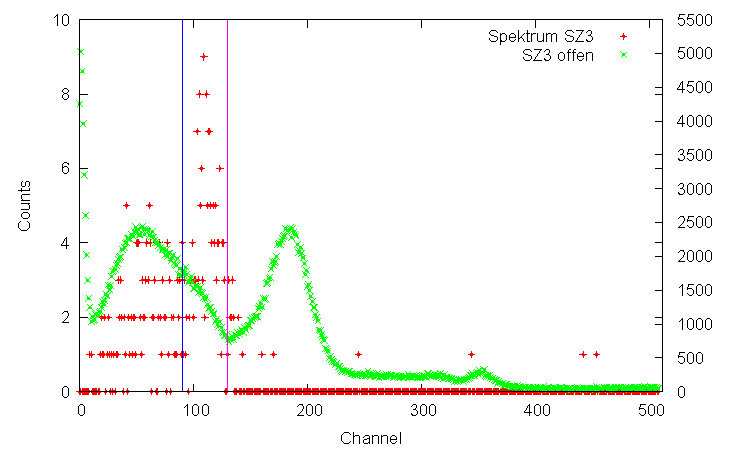
\includegraphics[width=\textwidth]{Graphen/quench/spektrum_3070.pdf}
 \caption{Spektrum 3070G}
\end{figure}

\begin{figure}
 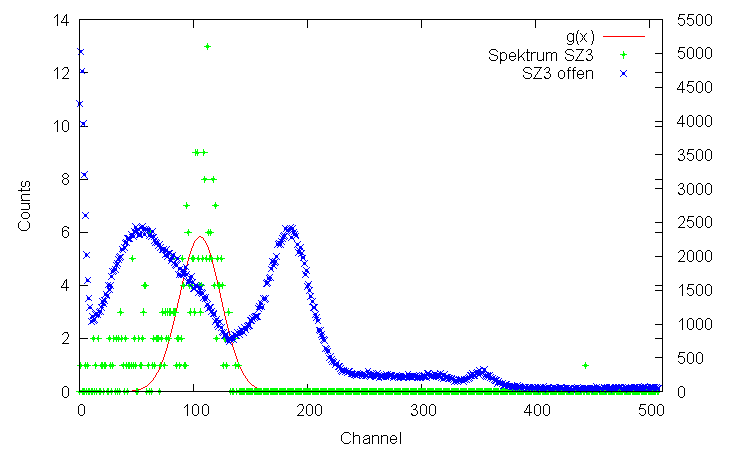
\includegraphics[width=\textwidth]{Graphen/quench/spektrum_4032.pdf}
 \caption{Spektrum 4032G}
\end{figure}

\begin{figure}
 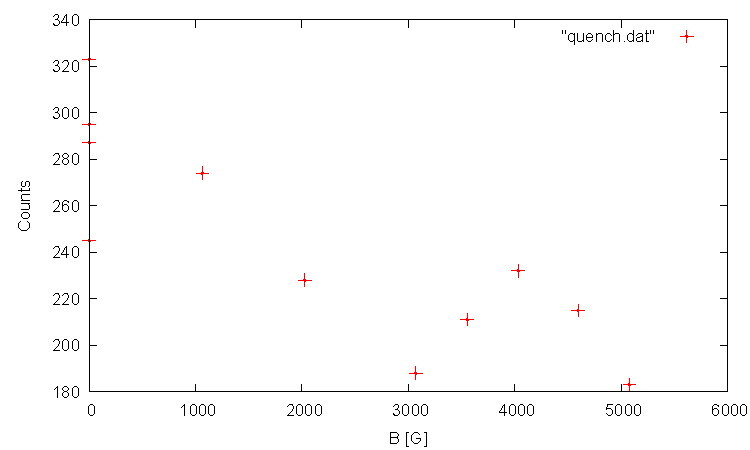
\includegraphics[width=\textwidth]{Auswertung/quench.pdf}
 \caption{Quenching des Drei-Photonen-Zerfalls in $120^\circ$-Konfiguration}
\end{figure}
Bei der Auswertung haben wir dann nur die Kanäle 90 bis 130 verwendet, was einem Energiefenster von bis %TODO: Eichung
entspricht. Die Ereignisse in diesem Intervall haben wir dann summiert und den Untergrund aus der Koinzidenzmessung abgezogen. Um die Schwankungen in der Apparatur auszugleichen, die uns die Kontrollmessungen zeigen, haben wir zur Normierung ein gewichtetes Mittel dieser verwendet.
\begin{equation*}
 N' = \frac{N}{2/3 N_{k1} + 1/3 N_{k2}}
\end{equation*}
Wobei $N_{k1}$ die zeitlich näherliegende Kontrollmessung bezeichnet und $N_{k2}$ die weiter entfernte. An die resultierenden Datenpunkte haben wir dann die Quenching-Funktion über den Parameter $\Delta W$ angepasst:
\begin{equation*}
 Q(B)/Q(0) = 0.5 + \frac{0.5}{1 + r \cdot ( \frac{2  \mu }{ \Delta W})^2 \cdot B^2} 
\end{equation*}


Im Graph (Abb \ref{auswertung-quench-normiert}) ist sowohl ein Fit an die Datenpunkte dargestellt, die über das gewichtete Mittel normiert wurden (f(x)) als auch ein Fit an Datenpunkte, die mit dem durchschnittlichen $Q(0)$ normiert wurden. 



\begin{figure}
 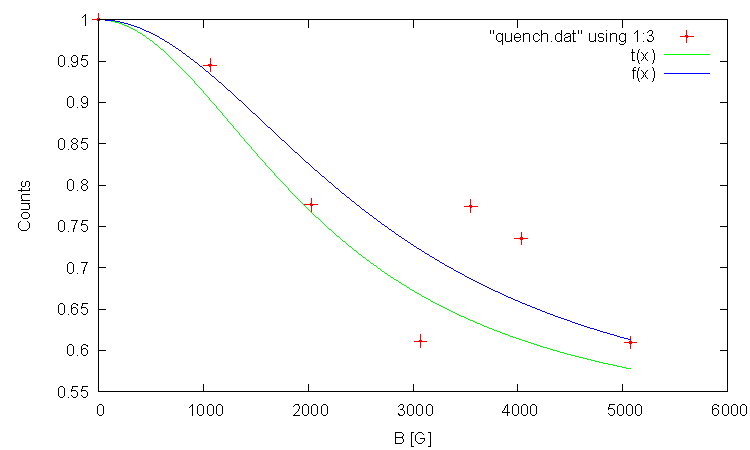
\includegraphics[width=\textwidth]{Auswertung/quench-normiert.pdf}
 \caption{Normiertes Quenching des Drei-Photonen-Zerfalls in $120^\circ$-Konfiguration}
 \label{auswertung-quench-normiert}
\end{figure}

Wir erhalten aus dem Fit folgenden Wert für die Feinstrukturaufspaltung:
\begin{equation*}
 \Delta W = (9,57758 \pm 1,593) \e{-4} eV
\end{equation*}

Der Literaturwert [TODO: Staatsexamensarb?] beträgt $\Delta W = 8,412\e{-4} eV$ und liegt also innerhalb der ersten Standartabweichung des von uns ermittelten Wertes. Die relativen Zählraten sind bei mehreren Einstellungen zu hoch. Dies deutet darauf hin, dass falsche Ereignisse registriert werden, also zB von 2-Photonen-Zerfällen, Bremsstrahlung oder auch Rauschen. Diese werden nicht vom Magnetfeld unterdrückt und führen somit zu einer zu großen Zählrate. Theoretisch ließen sich solche Ereignisse weiter reduzieren, indem engere Energiefenster und auch ein kleineres Koinzidenzintervall gewählt werden. Praktisch müsste dann allerdings die Meßzeit noch weiter verlängert werden, um statistisch relevante Ergebnisse zu erhalten. Da wir aber bereits so deutliche Drifts in den Messwerten sehen, scheint dies nicht sinnvoll. Besser wäre es sicherlich die \Na-Probe zu erneuern, wodurch sich ca. 100-fach höhere Zählraten ergeben würden (siehe \ref{verbleibende_aktivitaet}).